\section{State-Of-The-Art}
In this section related work and literature on the topic is discussed.

\subsection{Related Work}
While there is some literature available on component-based architectures, I am not aware of works that researched
moving from an inheritance based approach to a component based approach on the same product. I think this is the first
work describing the actual process. I am also not aware of any case studies of \OS{} real-time strategy game
architectures and object representation.

\subsection{Literature}
A small number of papers and books on the topic is available:
\begin{enumerate}
    \item A Generic Framework for Game Development - \cite{Fh02ageneric}
    \item A Software Architecture for Games - \cite{Doherty_2003}
    \item A flexible and expandable architecture for computer games - \cite{Plummer_2004}
    \item Game Architecture and Design: A New Edition - \cite{Rollings.2003}
\end{enumerate}

Most literature titled component-based embraces the use of components in a high level view. They define a component
as a library of classes that fulfilles a certain functionality (such as physics, AI or rendering), whereas I am
interested in the low level component design, where a component maps to a single class of functionality.

\cite{Rollings.2003} seperates between a hard and soft architecture. The hard architecture is the part of the
architecture that is platfrom or domain specific, whereas the soft architecture is usually mostly the game-logic itself.
In \cite{springerlink:10.1007/978-3-540-73551-95} Folmer gives a "Reference Architecture" for games, which can be seen in
\figref{fig:referencearch}. The soft archticture described in \cite{Rollings.2003} is only the \textit{Game Interface}
and \textit{Domain Specific} layers in this reference architecture, the rest is considered hard architecture. I am
interested in the components of the \textit{Game Interface} layer of the of soft-architecture, whereas most
research is done on the broad topic of the hard architecture or the \textit{Domain Specific} layer.

\begin{figure}[!htb]
\center
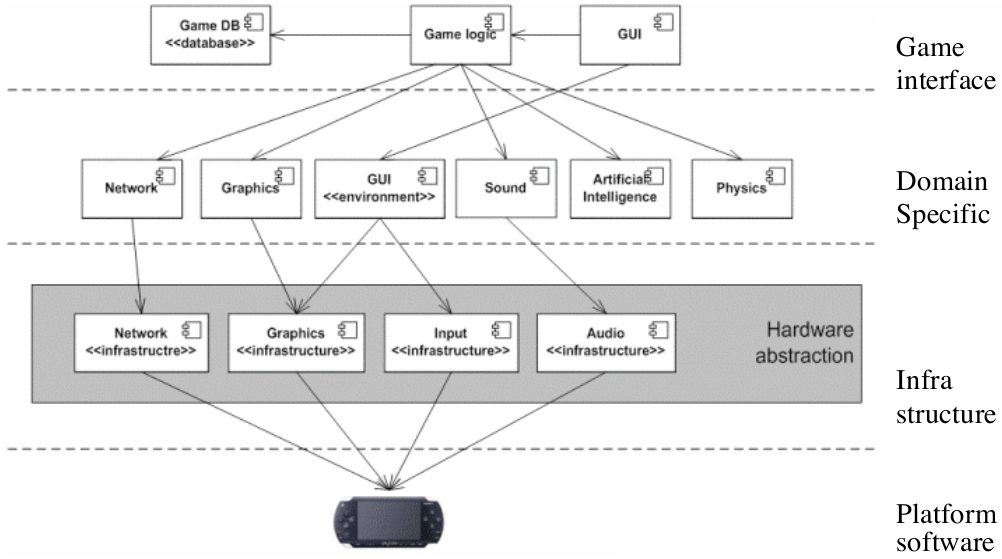
\includegraphics[scale=0.3]{pics/referencearch}
\caption{The reference architecture for games as given by Folmer -- graphic taken from the paper.}
\label{fig:referencearch}
\end{figure}

\cite{Rollings.2003} emphasizes the need for well thought-out interfaces between the components. So that for example a
route finding library/class can easily be exchanged for another one. Thus avoiding tight coupling between the high
level components where possible. He does not go into any deep details concerning components on the soft architecture
side, but he gives many ideas for design patters that can be used in game programming, such as the \textit{Singleton},
\textit{Factory} or \textit{Delegate} patters.
\linebreak

I found \citet{Fh02ageneric} particularly interesting, as it describes a system based only on components in great
detail. Haller not only explains the use of components, but also gives a very detailed proposition on how to handle
inter-component communication using a message system, based on and extending the QT GUI Framework\footnote{QT website:
\url{http://qt.nokia.com/}}.

Haller explains that components can be connected to each other using strictly typed in and outputs, making it possible to connect components
using an external (graphical) tool, easily usable by non-programmers. Having well defined in and outputs allows the
creation of component networks where as set of components are connected with each other over their in and
outputs. These networks can be looked at as a "meta-component" as the network has well defined in and outputs and can
thus itself be viewed as a component. Each component has a state in which it is in, when this state is changed a message
is sent through the outputs. The basic interface is given in \figref{fig:component}.

\begin{figure}[!htb]
\center
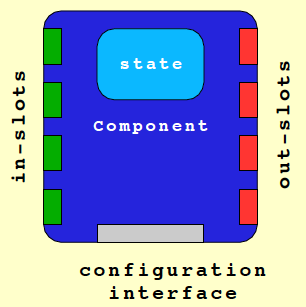
\includegraphics[scale=0.4]{pics/component}
\caption{The component interface as described by Haller \cite{Fh02ageneric} -- graphic taken from the paper.}
\label{fig:component}
\end{figure}

\cite{Doherty_2003} gives recommendations on how to structure a complete game-engine. He discusses the options of using
a component-based approach or a object-oriented design. He claimes one important advantage of using a component-based approach is:
\begin{quote}
It enforces a data-driven design philosophy. Since objects cannot be anything but data, all behavior must
be defined in terms of data. -- \cite[Page 4]{Doherty_2003}
\end{quote}
He argues this should be a favorable goal in the programming of a game, as it seperates the data from the code. By doing this it
ensures that game-designes can work in parallel with the programmers, but no recompiling of the software is needed to
change basic game attributes. Thus the teams productivity is improved.

He also brings arguments that favor the object-oriented system:
\begin{quote}
The internal representation matches the way that people think about the world. -- \cite[Page 4]{Doherty_2003}
\end{quote}

From reading his paper, I think he clearly favors the component-based approach. While acknoledging that it is more
difficult for the programmer to implement, it gives great benefitis for the game-designer. He claims that many problems
occuring with component-based systems can be solved using database proven concepts.



